\hypertarget{a00324}{}\section{Getting Started with A\+A\+X}
\label{a00324}\index{Getting Started with A\+A\+X@{Getting Started with A\+A\+X}}
A brief introduction to A\+A\+X. 

\hypertarget{a00324_aax_getting_started_guide_contents}{}\subsection{Contents}\label{a00324_aax_getting_started_guide_contents}
\begin{DoxyItemize}
\item \hyperlink{a00324_aax_sdk_guide_00_introduction}{Welcome} \item \hyperlink{a00324_aax_sdk_guide_01_aax_design_overview}{A\+A\+X Design Overview} \item \hyperlink{a00324_aax_sdk_guide_02_demogain_example}{Demo\+Gain Example}\end{DoxyItemize}
 \hypertarget{a00324_aax_sdk_guide_00_introduction}{}\subsection{Welcome}\label{a00324_aax_sdk_guide_00_introduction}
 Welcome to A\+A\+X! This guide is designed to introduce you to the fundamental concepts of A\+A\+X. By the end of this guide you will understand\+: \begin{DoxyItemize}
\item The purpose of A\+A\+X \item The basic components of an A\+A\+X plug-\/in \item The structure of the Demo\+Gain example plug-\/in\end{DoxyItemize}
If you would prefer to skip the documentation and jump straight to the code then we recommend jumping to \hyperlink{a00324_aax_sdk_guide_02_demogain_example}{Demo\+Gain Example} below. This section will walk you through the core parts of and A\+A\+X plug-\/in using the Demo\+Gain plug-\/in as an example. 

 \hypertarget{a00324_aax_sdk_guide_01_aax_design_overview}{}\subsection{A\+A\+X Design Overview}\label{a00324_aax_sdk_guide_01_aax_design_overview}
\hypertarget{a00324_subsection__architecture_philosophy}{}\subsubsection{Architecture Philosophy}\label{a00324_subsection__architecture_philosophy}
The purpose of the A\+A\+X architecture is to provide an {\itshape easy-\/to-\/use} framework for the development of {\itshape high-\/performance audio plug-\/ins} that can run on a {\itshape variety of platforms}, both present and future, with a {\itshape high level of code re-\/use}.

\hypertarget{a00324_subsection__design_attributes}{}\subsubsection{Design Attributes}\label{a00324_subsection__design_attributes}
A\+A\+X incorporates a flexible, decoupled component hierarchy, including\+: 
\begin{DoxyEnumerate}
\item A relocatable C-\/style callback that performs the plug-\/in\textquotesingle{}s real-\/time audio processing algorithm  
\item A collection of supporting C++ objects that manage the plug-\/in\textquotesingle{}s data, G\+U\+I, and any other non-\/real-\/time information  
\item A \char`\"{}description\char`\"{} method that statically describes the plug-\/in\textquotesingle{}s layout and compatibility requirements to the host.  
\end{DoxyEnumerate}

This flexible design facilitates optimal performance and portability; A\+A\+X is 64-\/bit ready and is designed to work well in both host-\/based (Native), accelerated (D\+S\+P), and future (e.\+g. embedded) environments. Importantly, plug-\/ins running in each of these environments can use the same code base, and porting to new platforms should not require much more than a re-\/compile. To satisfy these portability requirements, A\+A\+X must be decoupled into three parts, the G\+U\+I, data model, and algorithm.

\hypertarget{a00324_subsection__component_structure}{}\subsubsection{Component Structure}\label{a00324_subsection__component_structure}
The core component structure of an A\+A\+X plug-\/in involves data model, G\+U\+I, description, and algorithm modules. The design involves a mixture of C++ objects (data model and G\+U\+I modules) and C-\/style callbacks (algorithm and description modules.)

Figure shows basic object ownership and composition in an A\+A\+X plug-\/in. The purple components are provided as part of the A\+A\+X S\+D\+K while the gray components are written as needed by the plug-\/in developer. The classes above the dotted line are pure virtual interfaces, while the classes below the dotted line are concrete implementations.

  Figure 1\+: Core A\+A\+X interface design.

As you can see, the plug-\/in\textquotesingle{}s \hyperlink{a00328}{data model} and \hyperlink{a00329}{G\+U\+I} are written as C++ objects inherited from S\+D\+K interfaces, while its \hyperlink{a00327}{algorithm} and \hyperlink{a00326}{Description} methods are implemented as simple callbacks. This basic model may be expanded by attaching additional modules, such as the \hyperlink{a00334}{Host Processor} module used by advanced non-\/real-\/time plug-\/ins. In this section, however, we will be considering only the four core interfaces and modules.

\hypertarget{a00324_subsection__algorithm}{}\subsubsection{Algorithm}\label{a00324_subsection__algorithm}
The most fundamental, and most important, component of any audio plug-\/in is its processing algorithm. Due to the design requirements of an A\+A\+X plug-\/in, this component must meet several constraints in order to be compatible with accelerated platforms\+: 
\begin{DoxyEnumerate}
\item It must be possible to build the algorithm as a compatible component on a variety of platforms  
\item It must be possible for the host to re-\/locate the algorithm in memory without affecting the algorithm\textquotesingle{}s state  
\item The algorithm must be separable from the rest of its plug-\/in, e.\+g. into a different memory space  
\item The algorithm must be as efficient as possible to call.  
\end{DoxyEnumerate}

To satisfy these constraints, A\+A\+X uses a decoupled C-\/style callback function. State information within the function is obtained through the context, a custom data structure that contains everything from the \char`\"{}outside world\char`\"{} that is relevant to the algorithm. The context includes information such as audio buffers and coefficient packets, which are provided according to a static set of data routing definitions that we will describe further in the next chapter. The host is responsible for ensuring that this structure is up-\/to-\/date whenever the algorithm callback is entered.

\begin{DoxySeeAlso}{See also}
\hyperlink{a00327}{Real-\/time algorithm callback}
\end{DoxySeeAlso}
\hypertarget{a00324_subsection__data_model}{}\subsubsection{Data Model}\label{a00324_subsection__data_model}
The \hyperlink{a00099}{A\+A\+X\+\_\+\+I\+Effect\+Parameters} interface represents the data model portion of your plug-\/in. The A\+A\+X host interacts with your plug-\/in\textquotesingle{}s data model via this interface, which includes methods that store and update of your plug-\/in\textquotesingle{}s internal data.

In your plug-\/in\textquotesingle{}s data model implementation, you will be responsible for creating the plug-\/in\textquotesingle{}s parameters and defining how the plug-\/in will respond when these parameters are changed via control updates or preset loads. In order for information to be routed from the data model to the plug-\/in\textquotesingle{}s algorithm, the parameters that are created here must be registered with the host in the plug-\/in\textquotesingle{}s Description callback (see below).

The data model is composed with \hyperlink{a00090}{A\+A\+X\+\_\+\+I\+Controller}, an interface that provides access to the host. This interface provides a means of querying information from the host such as stem format or sample rate, and is also responsible for communication between the data model and the (decoupled) algorithm.

You will most likely inherit your custom data model\textquotesingle{}s implementation from \hyperlink{a00018}{A\+A\+X\+\_\+\+C\+Effect\+Parameters}, a default implementation of the \hyperlink{a00099}{A\+A\+X\+\_\+\+I\+Effect\+Parameters} interface. This class provides basic functionality such as adding custom parameters, setting control values, restoring state, generating coefficients, etc., which you can override and customize as needed.

 \begin{DoxySeeAlso}{See also}
\hyperlink{a00328}{Data model interface}
\end{DoxySeeAlso}
\hypertarget{a00324_subsection__gui_interface}{}\subsubsection{G\+U\+I Interface}\label{a00324_subsection__gui_interface}
The \hyperlink{a00098}{A\+A\+X\+\_\+\+I\+Effect\+G\+U\+I} interface contains the plug-\/in\textquotesingle{}s G\+U\+I methods. This interface is decoupled from the plug-\/in\textquotesingle{}s data model, allowing A\+A\+X to support distributed architectures that incorporate remote G\+U\+Is.

The G\+U\+I is also composed with \hyperlink{a00090}{A\+A\+X\+\_\+\+I\+Controller}, from which references to the plug-\/in\textquotesingle{}s other components, such as its data model interface, may be retrieved.

The A\+A\+X S\+D\+K includes a set of G\+U\+I extensions to help you get started implementing your plug-\/ins\textquotesingle{} G\+U\+Is. These extensions include both native drawing formats and suggested integrations with third-\/party graphics frameworks. Although the S\+D\+K does not include any actual graphics frameworks, these extensions provide examples of how you can incorporate your chosen G\+U\+I framework with \hyperlink{a00288}{A\+A\+X}.

 \begin{DoxySeeAlso}{See also}
\hyperlink{a00329}{G\+U\+I interface}
\end{DoxySeeAlso}
\hypertarget{a00324_subsection__describe}{}\subsubsection{Describe}\label{a00324_subsection__describe}
A plug-\/in\textquotesingle{}s Describe callback ties all the plug-\/in\textquotesingle{}s components together and registers the plug-\/in with the host. In this callback, your plug-\/in defines a set of algorithm callbacks, data connections, and static plug-\/in properties

In order to route data to the plug-\/in\textquotesingle{}s algorithm, Describe includes a description of the algorithm\textquotesingle{}s context structure. This description involves a set of port definitions, which can be \char`\"{}hard-\/wired\char`\"{} to receive data from the host (such as audio buffers,) from the plug-\/in\textquotesingle{}s data model (such as packets of coefficients,) or even from past calls to the algorithm (private, persistent algorithm state.)

Once these connections are made, Describe passes the host a populated description interface and returns. In the next section we will demonstrate how all these interfaces interact with one another by examining a sample plug-\/in.

\begin{DoxySeeAlso}{See also}
\hyperlink{a00326}{Description callback}
\end{DoxySeeAlso}
\hypertarget{a00324_subsection__controller}{}\subsubsection{Controller}\label{a00324_subsection__controller}
There is one additional core component to any A\+A\+X plug-\/in, the Controller. The plug-\/in does not implement this component -\/ rather, the Controller is an interface that provides access to various facilities provided by the host, as well as to the plug-\/in\textquotesingle{}s other modules. 

 \hypertarget{a00324_aax_sdk_guide_02_demogain_example}{}\subsection{Demo\+Gain Example}\label{a00324_aax_sdk_guide_02_demogain_example}
The A\+A\+X S\+D\+K includes a basic example plug-\/in named Demo\+Gain. In this section we will examine this plug-\/in to show how the various core modules in an A\+A\+X plug-\/in interact with one another. We will focus in particular on how the Demo\+Gain\textquotesingle{}s \char`\"{}gain\char`\"{} parameter is defined, routed to the algorithm, and used to apply a gain effect to audio samples.

 For a description of all the example plug-\/ins included in the S\+D\+K, see the \hyperlink{a00376}{Example Plug-\/\+Ins} page.

\hypertarget{a00324_subsection__getting_started_with_demogain}{}\subsubsection{Getting Started}\label{a00324_subsection__getting_started_with_demogain}
\hypertarget{a00324_subsubsection__build_the_aax_library}{}\paragraph{Build the A\+A\+X Library}\label{a00324_subsubsection__build_the_aax_library}
If this is your first time opening the A\+A\+X S\+D\+K then your first step should be to build the A\+A\+X Library project. The A\+A\+X Library is a static library containing default implementations of the A\+A\+X interface and convenience classes designed to make A\+A\+X development easy. All of the S\+D\+K example plug-\/ins link to this library, and your plug-\/ins should too.

Open the A\+A\+X Library project for your chosen I\+D\+E from the Libs/\+A\+A\+X\+Library directory and build the library. Now you are ready to build plug-\/ins!

\hypertarget{a00324_subsubsection__open_demogain}{}\paragraph{Open and build Demo\+Gain}\label{a00324_subsubsection__open_demogain}
The Demo\+Gain project is located in Example\+Plug\+Ins/\+Demo\+Gain. Once you have built the A\+A\+X Library project you will be able to successfully build Demo\+Gain.

\begin{DoxyNote}{Note}
To run Demo\+Gain or other example plug-\/ins in Pro Tools 10 you must change the {\ttfamily A\+A\+X\+\_\+e\+Plug\+In\+Category\+\_\+\+Example} category to {\ttfamily A\+A\+X\+\_\+e\+Plug\+In\+Category\+\_\+\+Dynamics} in the plug-\/in\textquotesingle{}s Describe function. The \char`\"{}example\char`\"{} category is not supported in Pro Tools 10.
\end{DoxyNote}
The Demo\+Gain plug-\/in that you just built is not digitally signed, so it will only run in a developer build of Pro Tools or in another host that does not require digital signatures for A\+A\+X plug-\/ins. If you have a developer build of Pro Tools then you can now test the plug-\/in by installing it and launching Pro Tools. See \hyperlink{a00360_subsection__install_directories_}{Install directories} section in the \hyperlink{a00360}{Pro Tools Guide} document for more information about installing A\+A\+X plug-\/ins for Pro Tools.

\hypertarget{a00324_subsubsection__now_what}{}\paragraph{Now what?}\label{a00324_subsubsection__now_what}
A good starting point for understanding a plug-\/in is to understand its parameters. In Demo\+Gain, as in most A\+A\+X plug-\/ins, the plug-\/in\textquotesingle{}s parameters define its data model state, and therefore the plug-\/in\textquotesingle{}s parameters provide the fundamental connection between user interactions and audio processing.

In the remainder of this section we will examine the gain parameter in Demo\+Gain to understand how this parameter is defined, hooked up, modified, and eventually applied to the plug-\/in algorithm. In this way we will \char`\"{}visit\char`\"{} each of the core design components in Demo\+Gain.

\hypertarget{a00324_subsection__overview_of_parameter_creation}{}\subsubsection{Overview of Parameter Creation}\label{a00324_subsection__overview_of_parameter_creation}
 To create a plug-\/in parameter, the following steps are required\+: 
\begin{DoxyEnumerate}
\item Data model\+: Create your parameter 
\begin{DoxyEnumerate}
\item Create a new parameter object  
\item Register the parameter with the Packet Dispatcher  
\item Create an update callback that converts the raw parameter value into a packet of processed coefficients  
\end{DoxyEnumerate}
\item Algorithm\+: Add new coefficients to the algorithm\textquotesingle{}s context structure 
\begin{DoxyEnumerate}
\item Create a new field for incoming coefficient packets  
\item Generate a {\itshape field I\+D} to reference the new member  
\item Add the new coefficient to the plug-\/in\textquotesingle{}s algorithm code  
\end{DoxyEnumerate}
\item Describe\+: Connect the parameter throughout the plug-\/in 
\begin{DoxyEnumerate}
\item Add a new Data Input Port to the algorithm via the component descriptor interface  
\item Add a connection between the parameter\textquotesingle{}s {\itshape packet I\+D} and its coefficients\textquotesingle{} {\itshape field I\+D} 
\end{DoxyEnumerate}
\item G\+U\+I\+: Add a control 
\begin{DoxyEnumerate}
\item Create a G\+U\+I widget that can update the parameter\textquotesingle{}s state  
\item Add logic to notify the data model when the G\+U\+I is edited  
\item Add logic to update the G\+U\+I when the data model state changes  
\end{DoxyEnumerate}
\end{DoxyEnumerate}

The following sections discuss these steps in greater detail, making use of the concrete implementation in {\itshape \hyperlink{a00018}{A\+A\+X\+\_\+\+C\+Effect\+Parameters}}.

\hypertarget{a00324_subsection__data_model_create_your_parameter}{}\subsubsection{Data Model\+: Create Your Parameter}\label{a00324_subsection__data_model_create_your_parameter}
Demo\+Gain\textquotesingle{}s data model inherits its functionality from \hyperlink{a00018}{A\+A\+X\+\_\+\+C\+Effect\+Parameters} (the default implementation of \hyperlink{a00099}{A\+A\+X\+\_\+\+I\+Effect\+Parameters}). The {\ttfamily Demo\+Gain\+\_\+\+Parameters.\+h} and {\ttfamily Demo\+Gain\+\_\+\+Parameters.\+cpp} source files comprise the source code for Demo\+Gain\textquotesingle{}s data model.

During plug-\/in initialization, {\ttfamily Demo\+Gain\+\_\+\+Parameters\+::\+Effect\+Init()} creates the plug-\/in\textquotesingle{}s custom parameters. A look inside of the .cpp file shows how this is done via the creation of a new \hyperlink{a00033}{A\+A\+X\+\_\+\+C\+Parameter} for the gain\+Parameter\+: the \hyperlink{a00033}{A\+A\+X\+\_\+\+C\+Parameter} constructor is parametrized with a set of arguments that define the gain parameter\textquotesingle{}s behavior, such as its default value ({\ttfamily 1.\+0f}), name (\char`\"{}\+Gain\char`\"{}), taper behavior (linear), etc.

After creating the parameter objects, a series of packets are registered with the host via the inherited \hyperlink{a00031}{Packet Dispatcher}, {\ttfamily m\+Packet\+Dispatcher}, which is a helper object used by \hyperlink{a00018}{A\+A\+X\+\_\+\+C\+Effect\+Parameters} to assist with the plug-\/in\textquotesingle{}s packet management tasks.


\begin{DoxyCode}
mPacketDispatcher.RegisterPacket(
    DemoGain\_GainID,
    eAlgPortID\_CoefsGainIn,
    \textcolor{keyword}{this},
    &DemoGain\_Parameters::UpdatePacket\_Gain); 
\end{DoxyCode}
  Listing 1\+: Registration of Demo\+Gain\textquotesingle{}s \char`\"{}gain\char`\"{} packet handler

The last parameter in \hyperlink{a00031_a1848f0bfa473b54e9ee8e32872c89cb1}{A\+A\+X\+\_\+\+C\+Packet\+Dispatcher\+::\+Register\+Packet()} takes a reference to a packet handler callback. This method will be called by the Packet Dispatcher whenever new parameter values need to be converted into coefficients that can be used by the algorithm. In Demo\+Gain, a reference to Demo\+Gain\+\_\+\+Parameters\+::\+Update\+Packet\+\_\+\+Gain() is used for the gain parameter\textquotesingle{}s coefficient packet.

As a developer, you will choose how this portion of your data model gets handled; you can choose to use the default handler method, which simply forwards the raw parameter values to the algorithm, or you can define a custom handler. You can also choose to bypass the Packet Dispatcher completely (see the {\ttfamily Demo\+Dist\+\_\+\+Gen\+Coef} plug-\/in for an example of this.)

Although the handling of Demo\+Gain\textquotesingle{}s gain parameter is trivial, for the sake of demonstration this plug-\/in uses both Packet Dispatcher approaches in the registration of its bypass and gain parameters.

\hypertarget{a00324_subsection__algorithm_add_coefficients_to_the_algorithms_context_structure}{}\subsubsection{Algorithm\+: Add coefficients to the algorithm\textquotesingle{}s context structure}\label{a00324_subsection__algorithm_add_coefficients_to_the_algorithms_context_structure}
 Your plug-\/in\textquotesingle{}s context is nothing more than a data structure of pointers that is registered with the host during Describe. These pointers function as {\itshape  ports} where host-\/managed data may be delivered or retrieved.

\hypertarget{a00324_subsubsection__context_definition_}{}\paragraph{Context definition}\label{a00324_subsubsection__context_definition_}


 Looking under the \char`\"{}\+Component context definitions\char`\"{} section within Demo\+Gain\+\_\+\+Alg.\+h, you will find Demo\+Gain\textquotesingle{}s {\ttfamily S\+Demo\+Gain\+\_\+\+Alg\+\_\+\+Context} context. This is Demo\+Gain\textquotesingle{}s context structure, and its sole purpose is to parametrize Demo\+Gain\textquotesingle{}s algorithm with a set of ports. Note the definition of a port for the gain coefficients that are created by {\ttfamily Demo\+Gain\+\_\+\+Parameters\+::\+Update\+Packet\+\_\+\+Gain()} and another port for the bypass value that is forwarded via the default packet update handler.




\begin{DoxyCode}
int32\_t               * mCtrlBypassP;
SDemoGain\_CoefsGain   * mCoefsGainP; 
\end{DoxyCode}
  Listing 2\+: Gain and bypass ports in the Demo\+Gain algorithm\textquotesingle{}s context structure

Once ports have been defined for the algorithm\textquotesingle{}s coefficients and other algorithmic data, unique identifiers for each port in the context must be generated. This is accomplished through use of the \hyperlink{a00149_acf807247ecd6e5899dc9dc31644e9a1d}{A\+A\+X\+\_\+\+F\+I\+E\+L\+D\+\_\+\+I\+N\+D\+E\+X} macro. The basic idea behind this macro is to generate I\+Ds that the host can use to directly address the ports within their context\+:


\begin{DoxyCode}
, eAlgPortID\_CoefsGainIn = \hyperlink{a00149_acf807247ecd6e5899dc9dc31644e9a1d}{AAX\_FIELD\_INDEX} ( SDemoGain\_Alg\_Context , mCoef ),
, eAlgFieldID\_AudioIn = \hyperlink{a00149_acf807247ecd6e5899dc9dc31644e9a1d}{AAX\_FIELD\_INDEX} ( SDemoGain\_Alg\_Context , mInputPP ) ) 
\end{DoxyCode}
  Listing 3\+: Some port I\+D definitions for the Demo\+Gain algorithm\textquotesingle{}s context structure

Now the context\textquotesingle{}s definition is complete. So far these are just fields in a struct; the host doesn\textquotesingle{}t yet know how to route packets from the data model to these ports. That information will come later, in the plug-\/in\textquotesingle{}s \hyperlink{a00324_subsection__describe_connect_the_parameter_throughout_the_plug-in}{description}. Once this context is described to the host, the host will know to populate it and pass it to the processing function located in Demo\+Gain\+\_\+\+Alg\+Proc.\+cpp.

\hypertarget{a00324_subsubsection__algorithm_processing_callback_}{}\paragraph{Algorithm processing callback}\label{a00324_subsubsection__algorithm_processing_callback_}



\begin{DoxyCode}
\textcolor{keywordtype}{void}
\hyperlink{a00149_aaa22112139aa627574b1ef562f579d43}{AAX\_CALLBACK}
DemoGain\_AlgorithmProcessFunction (
    SDemoGain\_Alg\_Context * \textcolor{keyword}{const} inInstancesBegin [],
    \textcolor{keyword}{const} \textcolor{keywordtype}{void} * inInstancesEnd ) 
\end{DoxyCode}
  Listing 4\+: The Demo\+Gain algorithm\textquotesingle{}s callback prototype

This is where the plug-\/in\textquotesingle{}s audio buffer processing of the plug-\/in occurs. Note that this function is passed a pointer to an array of {\ttfamily S\+Demo\+Gain\+\_\+\+Alg\+\_\+\+Contexts}. Each of these represents the state of a particular instance of Demo\+Gain, and contains pointers to the applicable coefficient and audio buffer data.

Using the {\ttfamily S\+Demo\+Gain\+\_\+\+Alg\+\_\+\+Context} array, instance-\/specific information and audio buffers are easily retrieved for processing. Demo\+Gain accomplishes this by first iterating over each plug-\/in instance, then over each channel, and finally over each sample, at which point the gain coefficient is applied to each sample in the input audio buffer and the sample data is copied to the output audio buffer\+:


\begin{DoxyCode}
\textcolor{comment}{// --------- Iterate over plug -in instances ---------//}
\textcolor{keywordflow}{for} (SDemoGain\_Alg\_Context * \textcolor{keyword}{const} * walk = inInstancesBegin ; walk &lt;
    inInstancesEnd ; ++ walk )
\{
        .
        .
        .
    \textcolor{comment}{// --------- Run processing loop over each input channel ---------//}
    \textcolor{comment}{//}
    \textcolor{keywordflow}{for} (\textcolor{keywordtype}{int} ch = 0; ch &lt; kNumChannelsIn ; ch ++)
    \{
        \textcolor{comment}{// --------- Run processing loop over each sample ---------//}
        \textcolor{comment}{//}
        \textcolor{keywordflow}{for} (\textcolor{keywordtype}{int} t = 0; t &lt; kAudioWindowSize ; t++)
        \{
                .
                .
                .
        pdO [t] = gain * pdI [t];
                .
                .
                .
        \} \textcolor{comment}{// Go to the next sample}
    \} \textcolor{comment}{// Go to next channel}
 \} \textcolor{comment}{// End instance-iteration loop }
\end{DoxyCode}
  Listing 5\+: Iterative loops in the Demo\+Gain algorithm

\hypertarget{a00324_subsection__describe_connect_the_parameter_throughout_the_plug-in}{}\subsubsection{Describe\+: Connect the parameter throughout the plug-\/in}\label{a00324_subsection__describe_connect_the_parameter_throughout_the_plug-in}
 As mentioned before, Describe provides a static description of all communication pathways between a plug-\/in\textquotesingle{}s algorithm, host, and data model. In addition, various effect properties are defined that help the host determine how to handle the plug-\/in.

Communication paths between the various plug-\/in components are described as connections between source and destination ports. In order for these communication paths to be created, the algorithm must first define some destination ports by actually registering its previously defined context fields as communication destinations. Demo\+Gain does this for its gain parameter through the following call to \hyperlink{a00088_a230293b9f6bb413626cd487ca501df75}{A\+A\+X\+\_\+\+I\+Component\+Descriptor\+::\+Add\+Data\+In\+Port()} in Demo\+Gain\+\_\+\+Describe.\+cpp\textquotesingle{}s {\ttfamily Describe\+Algorithm\+Component()} method\+:


\begin{DoxyCode}
\hyperlink{a00088}{AAX\_IComponentDescriptor} * compDesc;
compDesc = outDescriptor->NewComponentDescriptor ();
err = compDesc->\hyperlink{a00088_a230293b9f6bb413626cd487ca501df75}{AddDataInPort} (
    eAlgPortID\_CoefsGainIn ,
    \textcolor{keyword}{sizeof} (SDemoGain\_CoefsGain) ); 
\end{DoxyCode}
  Listing 6\+: Adding a data port to Demo\+Gain\textquotesingle{}s algorithm component descriptor

This registration process is required for both custom coefficients (Gain) and for data that all plug-\/ins need such as audio input and output fields.

That completes the connection, and now the plug-\/in is fully wired to receive parameter updates, convert raw parameter values to algorithmic coefficients, pack these coefficients into a packet, post the packet to the host for routing, receive the updated packet in the list of context structures that the host provides when calling the algorithm callback, and apply the updated coefficient data in the appropriate context structure to the plug-\/in\textquotesingle{}s audio data. Whew! \hypertarget{a00324_subsection__gui_add_a_control}{}\subsubsection{G\+U\+I\+: Add a control}\label{a00324_subsection__gui_add_a_control}
 Although the specific steps for adding a G\+U\+I control to edit a plug-\/in parameter will vary depending on the G\+U\+I framework you choose, there are a few basic design principles that should always be followed.

The basic Demo\+Gain plug-\/in does not include any G\+U\+I implementation. For practical G\+U\+I implementation examples, open the Demo\+Gain\+\_\+\+G\+U\+I\+Extensions sample plug-\/ins. Demo\+Gain\+\_\+\+Cocoa provides an example of a custom plug-\/in G\+U\+I using the native O\+S X S\+D\+K, while Demo\+Gain\+\_\+\+Win32 uses native Windows A\+P\+Is. The other examples in this folder require common third-\/party libraries.

\hypertarget{a00324_subsubsection__control_edits_vs_parameter_updates_}{}\paragraph{Control edits vs. parameter updates}\label{a00324_subsubsection__control_edits_vs_parameter_updates_}
 The most important principle for A\+A\+X G\+U\+I design is that an edit in a plug-\/in\textquotesingle{}s G\+U\+I should never directly set the state of the associated parameter or parameters. This is because there may be other controller clients of the plug-\/in\textquotesingle{}s data model which will need to be notified of the edit, or which may need to override edits from the G\+U\+I. 
\begin{DoxyItemize}
\item  On control edit

When a control is edited in the plug-\/in G\+U\+I, call \hyperlink{a00061_a368b0f5a761d1eda4c41b420f153a077}{A\+A\+X\+\_\+\+I\+Effect\+Parameters\+::\+Set\+Parameter\+Normalized\+Value()}. The implementation of this method should post a request to the host in order to trigger the parameter update. The G\+U\+I should not update its state until the corresponding parameter update notification is received.  
\item  On parameter update

A parameter update can occur in response to a G\+U\+I edit, an edit from another attached controller, an update to a linked parameter, or any other event that affects the state of the data model. When the state of a parameter changes, \hyperlink{a00060_a45b468fef806611581f748af9301ab4d}{A\+A\+X\+\_\+\+I\+Effect\+G\+U\+I\+::\+Parameter\+Updated()} is called. The plug-\/in\textquotesingle{}s G\+U\+I should be updated in this method in order to reflect the new state of the affected parameter.  
\end{DoxyItemize}

For detailed information about the sequence of events and G\+U\+I responsibilities during a parameter update, see \hyperlink{a00350}{Parameter updates}

\hypertarget{a00324_subsubsection__notifying_the_host_of_gui_events_}{}\paragraph{Notifying the host of G\+U\+I events}\label{a00324_subsubsection__notifying_the_host_of_gui_events_}
 Some G\+U\+I events must be handled by the host rather than by the plug-\/in. For example, in Pro Tools a user should be able to display a pop-\/up menu for controlling automation information by command-\/option-\/control-\/clicking (Mac) or alt-\/ctl-\/right clicking (Windows) a control. These events, and other direct communication between the G\+U\+I and the \char`\"{}container\char`\"{} in which the host creates the plug-\/in view, is accomplished via the \hyperlink{a00117}{A\+A\+X\+\_\+\+I\+View\+Container} interface. Be sure to always call the handler methods in this interface before handling a mouse event within the plug-\/in G\+U\+I, in order to maintain the expected host behavior.

 Collaboration diagram for Getting Started with A\+A\+X\+:
\nopagebreak
\begin{figure}[H]
\begin{center}
\leavevmode
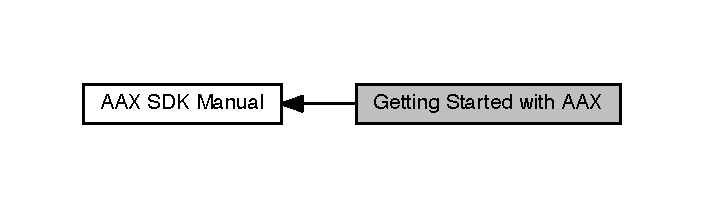
\includegraphics[width=338pt]{a00324}
\end{center}
\end{figure}
